\documentclass[a4paper,12pt]{jsbook}
\usepackage[utf8]{inputenc}
\usepackage[dvipdfmx]{graphicx}
\usepackage{url}
\usepackage{listings}
\usepackage{comment}

\fboxsep=0pt  %画像と枠線をくっつける。
\fboxrule=1pt %枠線の太さを1ptにする。
\begin{document}

\author{藤井 恵介}
\title{情報基礎演習(工学部)}
\date{2016年7月11日}

\frontmatter
\maketitle
\tableofcontents

\mainmatter
\chapter{ガイダンス}

\section{はじめに}
パソコン(Personal Computer) は、文字通りパーソナル・個人的に一人で一台を独占して利用することを前提に作られている。
例えば、あなたが友達のパソコンを使う機会があったとする。
あなたが昨日、自分のパソコンで作った文章を友達のパソコン上でちょっと編集して新しい文章を作りたいと思ったとしても、
あなたのパソコンは遠く離れたあなたの家にあり、わざわざ家に帰って、CD や USB メモリに保存し、もう一度持ってこなくてはならない。

これに対してメディアセンターには、一つの部屋に何台ものパソコンが並んでいる。例えば、この演習室には約60台のパソコンが並んでいる。
仮に、これらのパソコンにNo. 1 から順に番号をつけるとする。ある日、あなたが No. 7 のパソコンを使って、自分宛の電子メールを読んだり、ワープロでレポートを書いたりしたとすると、このときのデータはNo. 7 のパソコン上に保存され(るように見え)る。次の日にあなたが演習室に来てみると、No. 7 のパソコンはすでに他の人に使われていた。
このような時でも、No. 7 のパソコン上に保存した(ように見えた)あなたの電子メールは他人に読まれることはないし、レポートの続きを書くためにNo. 7 のパソコンが空くまで待つ必要もない。演習室の別のパソコン、例えば、No. 51 のパソコンを使って、続きの作業をすることができる。
これが、メディアセンターのパソコンの最大の特徴である。あたかも、自分一人だけのパソコンのように内容の秘密を保ちながら、どのパソコンを使っても同様の作業環境が提供されている。この特徴は、この演習室内のパソコンにとどまらず、大学内のあちこちに設置されているメディアセンターすべてのパソコンについて実現されている。このようなパソコンをPC端末と言う。

PC端末(教育用コンピュータシステム)の基本的な使い方は、京都大学情報環境機構のホームページに「学生のための情報環境活用マニュアル」(pdf ファイル)があるので、これを参照してもよい。

\url{http://www.iimc.kyoto-u.ac.jp/ja/services/ecs/support/tebiki.html}

このような環境を実現するために、メディアセンターではサーバと呼ばれる大きな一つのパソコンに各PC端末がつながっているシステムを形成している。
そのため、システムを利用する際、これから No. 51 のパソコンを使うのは「あなた」だということを知らせる必要がある。
これをログオンと言う。
また、使い終わった時には、今後このPC端末を使うのはもはやあなたではないことを知らせる(ログオフ)必要がある。
これは、他人にあなたのデータを悪用されないようにするためである。 ログオンの際には、利用コード(ID)と本人しか知らないパスワードが必要である。

パスワードは絶対に忘れないように、また、他人に教えるのはもちろん、不意に知れたりしないようにくれぐれも気をつけること。
これらパスワードの注意事項に関しては「学生のための情報環境活用マニュアル」の3.情報システムの安全で適正な利用のお願いに記載されているので、熟読しておくこと。
また、万が一利用コードやパスワードを忘れた場合は、学生証を持ってメディアセンター南館事務室で手続きをする。
 
\section{情報基礎演習の講義目標}
情報基礎演習では、これから大学生活に必要なワードプロセッサ(ワープロ)、表計算のほか、
実験や演習などのレポートや卒業論文の作成にに必要不可欠なプログラミングスキルを養う。

\section{成績評価およびテキストについて}
成績評価に際しては課題提出を評価する。試験は行わない。
演習内容はシラバスに準ずるが、クラスごとに若干異なる。
テキストは、京都大学情報環境機構のPandA(https://panda.ecs.kyoto-u.ac.jp/portal)上の講義HPに掲載している。
PandAにはECS-IDを使用してログインする(「a001…」のID)。

\begin{figure}
\centering
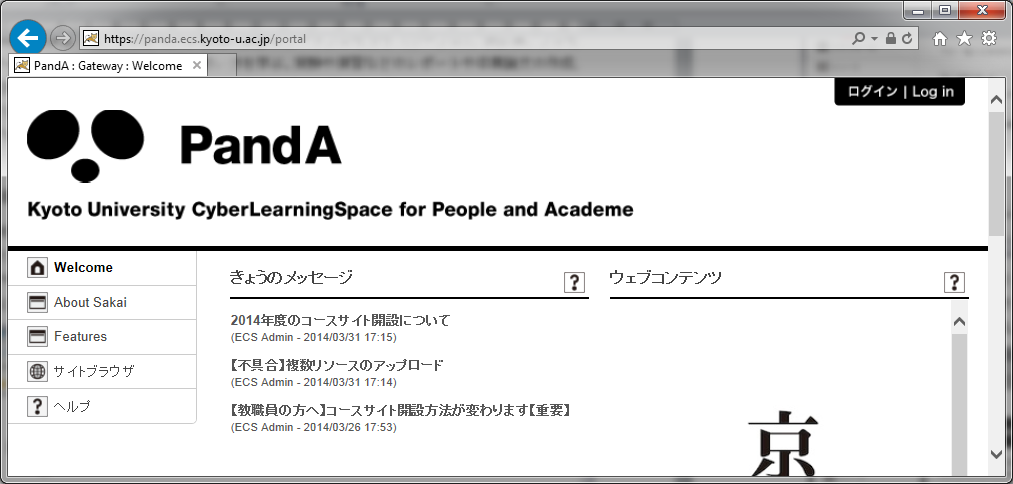
\includegraphics[width=13cm]{TeX_files/figs1/PandA1.png}
\caption{
\label{fig:PandA1}
PandA ログイン画面。右上のログインをクリックし、ECS-IDおよびパスワードを入力してログインする。}
\end{figure}

\begin{figure}
\centering
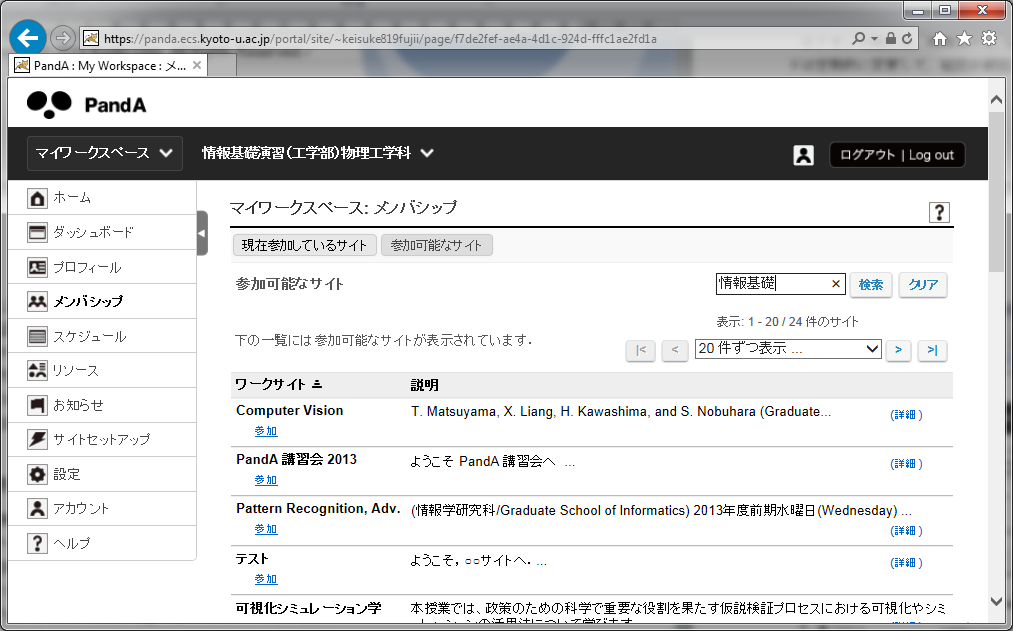
\includegraphics[width=13cm]{TeX_files/figs1/PandA2.png}
\caption{
\label{fig:PandA2}
左の欄の「メンバシップ」をクリックし、次に画面上部の「参加可能なサイト」をクリックしてワークサイトの一覧を表示させる。
一覧から「情報基礎(工学部)物理工学科」を探し(検索も可能)、「参加」をクリックする。}
\end{figure}

\begin{figure}
\centering
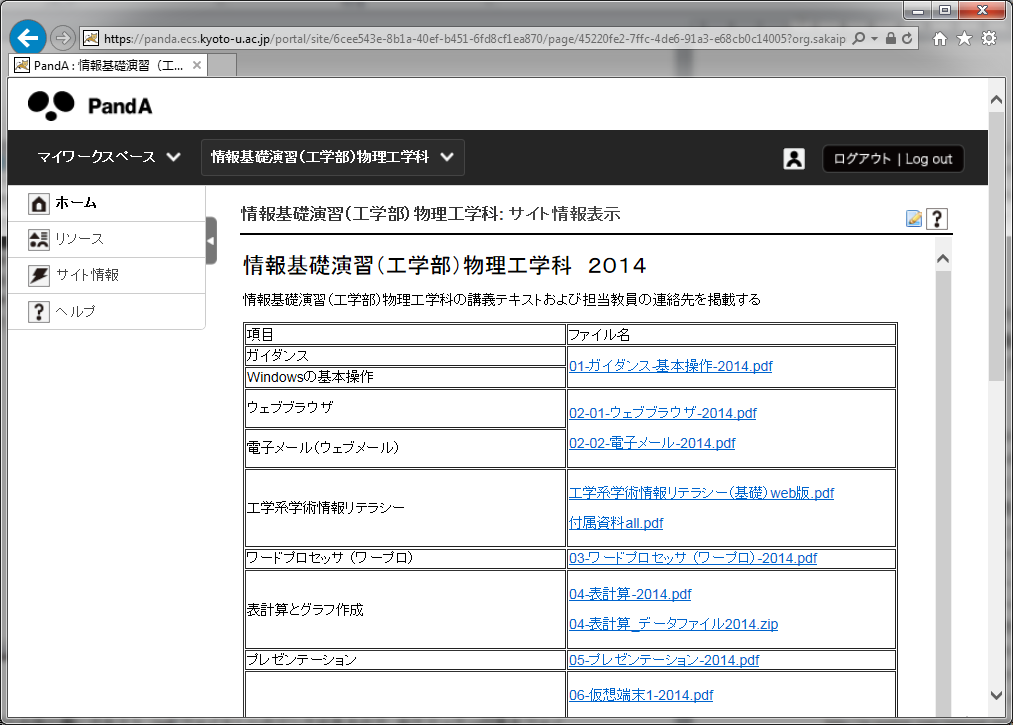
\includegraphics[width=13cm]{TeX_files/figs1/PandA3.png}
\caption{
\label{fig:PandA3}
表の右側の欄にテキスト (pdfファイル) へのリンクがあるので、右クリック→対象をファイルに保存で自分のMドライブ(マイドキュメントフォルダ)に保存しておくとよい。また次回からは、講義HPのURL
https://panda.ecs.kyoto-u.ac.jp/portal/site/6cee543e-8b1a-40ef-b451-6fd8cf1ea870/
をブラウザに入力し、PandAにログインすると、テキスト掲載ページが表示される。
}\end{figure}

 
講義中に分からないことはその時にどんどん質問すること。担当教員以外にもTA(ティーチングアシスタント)と呼ばれる大学院生(あなたたちの先輩)もいる。
 
\section{学術情報メディアセンター利用案内}
メディアセンターのPC端末は授業とは関わりなく全学生が利用可能である。
PC端末が設置してある場所は「学生のための情報環境活用マニュアル」の付録-5.サテライト配置図(最後のページ)に掲載してある。
「情報基礎演習」以外にもメディアセンターのPC端末を利用して行われる授業があり、また、直接授業では利用しなくても、レポートや課題の作成にPC端末のワープロや計算ソフトなどの利用を前提としている講義もある。
OSはWindows 7を搭載しており、ワープロソフトや表計算ソフトだけでなく、数式処理システムソフトや統計解析ソフト、プログラミング支援ソフトなどがインストールされている。
また、それぞれの部屋に設置されているプリンタを使って作成した文書等を印刷することができる。(一人当たり年間200枚の出力制限有り)
 
\section{利用に関しての注意}
PC端末を利用する際の注意に関しては、「学生のための情報環境活用マニュアル」の3.情報システムの安全で適正な利用のお願いおよび4.PC端末サービスの利用方法に記載してあるので、熟読すること。
中でも以下のことに特に気をつけること。
\begin{enumerate}
\item パスワードの適切な管理

\item コンピュータウィルスへの注意

・ 不審なメールを絶対に開かない。

・ 怪しい Web サイトには行かない。

・ 出所のはっきりしないファイルを開かない。

\item  自身のパソコンのセキュリティ対策
 利用者自身が持っているパソコンについても以下のセキュリティ対策をすること。

・ Windows や Office などソフトウェアは常に最新の修正プログラムを適用する。

・ ウィルス対策ソフトを導入し、常に最新のウィルス定義ファイルに更新する。

・ 自宅などでのネットワークへの接続では、ファイアウォールの設定やインターネットセキュリティソフトなどにより安全性の高い接続を確保する。

・ ウィルス対策、およびインターネットセキュリティの両方の機能を備えたソフトウェアが販売、または配布されているので利用するとよい。

シマンテック インターネットセキュリティ(有料)

\url{http://jp.norton.com/internet-security}

トレンドマイクロ ウイルスバスター(有料)

\url{http://safe.trendmicro.jp/purchase/vb.aspx/}

キングソフト インターネットセキュリティ(無料)

\url{http://www.kingsoft.jp/is/index.html}

アバスト! アンチウイルス(無料)

\url{http://www.avast.co.jp/index}
\end{enumerate}

\section{ファイル交換ソフトの使用禁止}
Winny, WinMX, Shareなどのファイル交換ソフトは著作権等の問題となっている。
そのため、PC端末におけるファイル交換ソフトの使用は禁止する。使用できないソフトウェアについては、「学生のための情報環境活用マニュアル」3.4 ネットワーク利用上の注意を参照。
P2Pシステムの使用禁止

Skype などの P2P システムについても、メディアセンターの PC端末では使用を原則禁止します。

その他、疑問点については「学生のための情報環境活用マニュアル」の付録(45ページ~)を参照するか、担当教員に相談する、もしくはメディアセンターに連絡する。


メディアセンター(情報環境機構)の連絡先

075-753-7400

URL:https://www.iimc.kyoto-u.ac.jp/ja/inquiry/
 
 
平成28年度情報基礎演習 担当教員

藤井 恵介(ふじい けいすけ)	\url{fujii_at_me.kyoto-u.ac.jp}

安部 豊(あべ ゆたか) \url{yutaka_abe_at_nucleng.kyoto-u.ac.jp}

沖野 真也(おきの しんや)\url{okino.shinya.8n_at_kyoto-u.ac.jp}

池之上 卓己(いけのうえ たくみ) \url{ikenoue.takumi.4m_at_kyoto-u.ac.jp}

市川 和秀(いちかわ かずひで) \url{kazuhide_at_me.kyoto-u.ac.jp}

\section{補足1. パソコンを買う際のアドバイス}
上にあるように、PC端末にはワープロソフト、表計算ソフトおよびプレゼンテーションソフトがインストールされている。
これら3つのソフトは今後もよく利用するので、家のパソコンにもインストールしておくとよい。
特に、これから新しいパソコンを買う際、ワープロソフト、表計算ソフト(MicrosoftでいうWordとExcel)は一緒についてくるパッケージが多いが、プレゼンテーションソフト(Powerpoint)は最小パッケージにはついていない可能性が高いので、プレゼンテーションソフト付きのパッケージを購入するとよい。
(Microsoft にもOffice Personal with PowerpointやOffice Standardなどのパッケージがある。)
後から、プレゼンテーションソフトのみを買うと価格が高い。

\section{補足2. WindowsとMac}
現在販売されているパソコンは、OSの種類によって大きく2つに分けられる。
WindowsとMacである。パナソニックなどの日本のメーカが販売しているパソコンにはWindows(Microsoft製OS)がインストールされている。
一方、iPhone等で知られるApple Computer から販売されているものが(通称)Macである。
世界のユーザーの9割以上がWindowsユーザーと言われているので、通常はWindowsを購入する方が良い。
一部のマニアックな人々(大学の先生やクリエイターと呼ばれる人たちなど)はMacを使っている。

\chapter{Windowsの基本操作}

\section{ウェブブラウザ}
\subsection{ウェブブラウザとインターネット}
Windowsには Internet Explorerというブラウザがデフォルトでインストールされている。
また、京都大学のPC端末にはMozilla Firefox というブラウザもインストールされている。
両者の基本機能は同じであるが、使い勝手が少し異なる。好みのものを利用すること。

ブラウザの上の方には、閲覧しているウェブサイトのURL (Uniform Resource Locator, 通称、アドレス)が記載してある。
URL の最後は意味があり、最後の2文字は
\begin{itemize}
\item \url{jp} = 日本、
\item \url{uk} = イギリス、
\item \url{fr} = フランス、
\item \url{de} = ドイツ、
\end{itemize}
など、国の名前に対応しており、その前の2文字は
\begin{itemize}
\item \url{co} = 企業、
\item \url{ac} = 大学・研究機関、
\item \url{go} = 政府機関、
\item \url{ne} = 通信関係、
\item \url{or} = その他の機関
\end{itemize}
など、組織の種別に対応している。
ただし、アメリカだけは特別で、国名に当たる部分は省略した上で、最後を3文字で表記することになっている。この3文字はそれぞれ
\begin{itemize}
\item \url{com} = 企業
\item \url{edu} = 大学・研究機関
\item \url{gov} = 政府機関
\item \url{net} = 通信関係
\item \url{org} = その他の機関
\end{itemize}
などのように対応している。

\subsubsection{課題}
\begin{enumerate}
\item ブラウザ(Internet Explorer)を起動する。(デスクトップにあるアイコンをダブルクリック)
\item 京都大学内のホームページ(HP)を知る。

   →京都大学のHP (http://www.kyoto-u.ac.jp/ja) を開く。

   →お気に入りに追加する。
\item 上の「教育・学生支援」にカーソルを合わせるとでてくる「その他学生生活支援」をクリックする。
\item 生活面の諸注意の中の「諸注意」をクリックし、サイト内の情報を熟読すること。
\end{enumerate}

\subsection{違法コピー・ダウンロードの禁止(重要!!)}
サイト上の絵や写真、音楽、映像などを著作権者の許可なく無断でコピー、ダウンロードすることは著作権法に違反し、10年以下の懲役または1,000万円以下の罰金が科せられる。
これまでは、私的利用に限りコピーやダウンロードが認められてきたが、平成22年1月1日に改正著作権法が施行され、たとえ私的であっても違法にアップロードされたものをダウンロードできなくなった。
例えば、YouTube などでテレビドラマなどを見ることも違法となるので、注意すること!!
特に、京都府警のサイバーポリスは優秀で、過去に何人も摘発されている。

違法コピー・ダウンロードはしない!

\subsection{e-learning による情報倫理の学習}
Web は非常に便利なものであるが、ルールを守って使用する義務がある。
つまり、「情報倫理」をきちんと学ぶ必要がある。
京都大学では、e-learning による情報倫理学習コンテンツを国立情報学研究所(NII)が提供する『学認連携 Moodle 講習サイト』により提供している。
デスクトップのショートカット、又は下記の URL から 教育用計算機システムの ID およびパスワードを入力し、ログインする。「学生のための情報環境活用マニュアル」も参照。
\url{http://www.iimc.kyoto-u.ac.jp/ja/services/ismo/e-Learning/}

\subsubsection{課題6}
京都大学情報システム利用規則とセキュリティのテキスト教材で学習したのち、修了テストを行い、その修了画面をPrtScr を使ってコピーしなさい。
次に、スタート→すべてのプログラム→アクセサリ→ペイントでペイントを立ち上げる。
そこに、コピーした画像をペーストし、rinri2015-00000000.jpg というファイル名を付けて M ドライブに保存しなさい。(00000000 の部分には学籍番号を入れること。)

補足:PrtScr は画面全体をコピーすることができる。アクティブな画面のみをコピーしたい場合は、Alt + PrtScr を使うとよい。

\begin{figure}
\centering
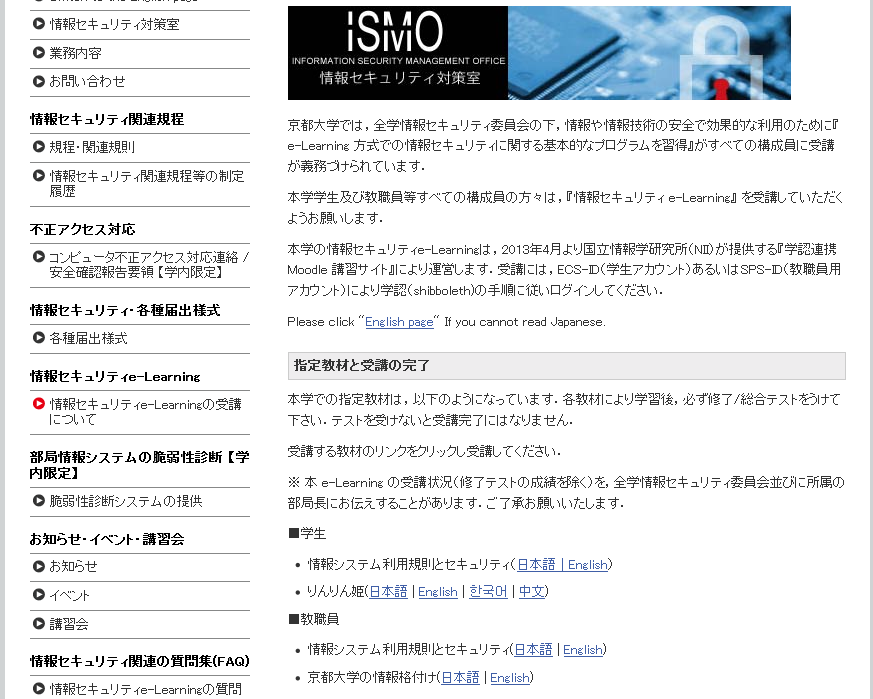
\includegraphics[width=13cm]{TeX_files/figs2/e-learning.png}
\caption{
\label{fig:e-learning}
e-learningへのリンク。右側下部の 学生 > 情報システム利用規則とセキュリティ をクリックする。
}
\end{figure}

\section{電子メール(ウェブメール)}
\subsection{はじめに}
最近は、Lineなどインスタント・メッセンジャーが広く利用されているが、
大学や会社などでは電子メールは一つの公式な文書である。
そのため、ここでは京都大学が提供する電子メールサービスである KUMOI の使い方を学ぶとともに、電子メールを送る際のマナーについても学ぶ。

\subsection{KUMOI}
京都大学情報環境機構ではMicrosoft社が運営するOffice365(Microsoft Office 365 for education)を活用した電子メールサービスを提供している。
これは京都大学に在籍する人は、申請すれば誰でも使用できるので利用するとよい(みなさんはすでに申請済みのはずである)。
ウェブメールは学外(家など)からもメールの受信・送信ができるので便利である。
Internet Explorer もしくは Mozilla Firefox をダブルクリックし、下記のURLを入力し、KUMOI のログイン画面を開く。 

\url{https://mail.st.kyoto-u.ac.jp/LiveLogin/}

ECS-ID、パスワードを入力し、ログインする(詳細は「学生のための情報環境活用マニュアル」8.学生用電子メールサービスの利用方法を参照。)

\begin{figure}
\centering
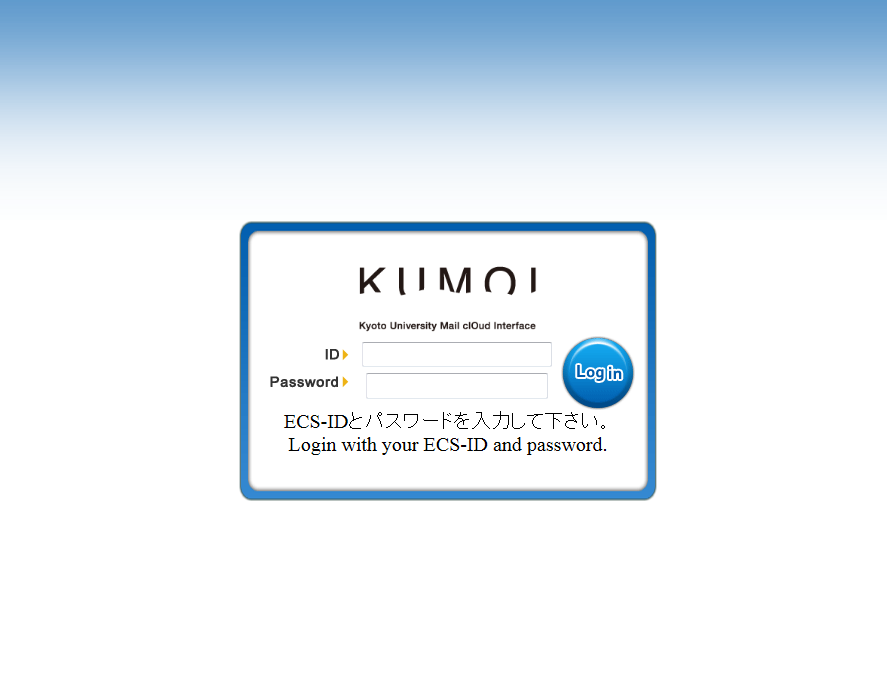
\includegraphics[width=13cm]{TeX_files/figs2/Kumoi.png}
\caption{
\label{fig:Kumoi}
e-learningへのリンク。右側下部の 学生 > 情報システム利用規則とセキュリティ をクリックする。
}
\end{figure}

\subsection{署名}
 電子メールには「署名」という機能がある。署名には名前や連絡先を記載し、一度作成して設定しておけば、送信するメールに自動的に添付されるので便利である。

\begin{enumerate}
\item KUMOIの(オプション)→(すべてのオプションを表示)→(設定)→(メール)と移動し、(電子メールの署名)ボックスに署名を入力する。。

<署名の例>

**********************

 京都大学工学部 物理工学科 1回生 T09

 藤井 恵介 (ふじい けいすけ)

 学籍番号:0000000000

E-mail::xxxxxxxx@st.kyoto-u.ac.jp

**********************

\item 送信メッセージに自動的に署名を追加する)チェックボックスをオンにする(これを忘れると、署名が添付されない。)
\end{enumerate}

\subsection{電子メールにおけるマナー}
電子メールは一種の手紙であるので、Lineのメッセージように宛名等を省いて、用件だけ書くようなことはしない。
電子メールのマナーについては、特に下記の事に気を付けること。
\begin{itemize}
\item 差出人を明らかにする。
\item 件名を必ず書く。
\item 本文の始めに誰に宛てたメールかを必ず書く。
\item 段落が変わるような場所には1行空行をはさむ。
\item 丁寧な言葉づかいを心がける。特に、目上の人には気を付ける。

<例>

○○先生

(1行あける)

物理工学科1回生の××です。

情報基礎演習の課題をお送りします。

よろしくお願いいたします。

\item あまり大きなサイズの添付ファイルを送らない。(京都大学のサーバは10MB程度なら送ることができるが、相手が受け取れない可能性がある。)
\item 相手が表示できる形式のファイルで送信する。(pdf ファイルであれば問題ない。)
\item パスワード、クレジットカード番号などの機密情報は電子メールに記載しない。

\end{itemize}

\subsubsection{【課題1】}
上の手順に従って、自分の署名を作成せよ。署名には名前、ふりがな、学籍番号、クラス、メールアドレスを記載すること。作成が終わったら、送信メールに署名を追加するのを忘れないようにすること。次に、メールを作成し、隣の人にメールを送ってみよ。件名、宛名等を必ず書くこと。本文に作成した署名が入っていることを確認すること。メールを受け取ったら、隣の人に返信してみよ。(返事を書いて送る。)

\subsubsection{【課題2】}
間違ったアドレスに(例えば、自分のアドレスの最後のjpを消して)メールを送ってみよ。しばらくすると、MAILER-DAEMON@MAILER-DAEMON という差出人からエラーメッセージが届くことを確認せよ。
このメールが送られてきた場合は、相手にメールが届いていないので、アドレス等を確認してメールを送り直す必要がある。


\subsubsection{【課題3】}
Web上での情報検索を駆使して、以下の問に答えよ。
解答の作成にはメモ帳を利用し、ファイル名は kadai110407-00000000.txt とすること。110407 の部分には今日の日付を、00000000 の部分は自分の学籍番号を入れること。

問1)現在の京都大学総長のフルネームは?

問2)京都大学の創設は何年?

問3)平成28年度前期の試験期間はいつからいつまでか?

問4)京都大学にある学部を全て答えよ。

問5)現在のアメリカ大統領、バラク・オバマの実父はどこの国の出身?

問6)USBメモリのUSBとは何の略?

問7)「ナノ」とは10の何乗のこと?

問8)プランク定数の値は?(単位とともに答えよ。)

問9)銀閣寺および金閣寺の正式名はそれぞれ何か?

問10)マイクロソフトの本社は何州何市にあるか?

\chapter{Microsoft Word}

\section{はじめに}
ワープロは文章を作成するアプリケーションである。
文字の属性(フォント、大きさ、文字飾り)の指定、図表の取り込みなどが可能であり、レイアウトの最終形を見ながら作業を行い、印刷することを目的としている。

演習室で使用するパソコンには、ワープロソフトとして、Microsoft Officeの「Microsoft Word 2010」とLibre Officeの「Writer」がインストールされている。
Microsoft Wordは、マイクロソフトがWindows及びMac OS X向けに販売している文書作成ソフトウェアであり、表計算ソフトウェアExcelとともにMicrosoft Officeの中核をなすアプリケーションである。
一般的にMicrosoft Wordはワード(WordまたはMS-Word)と呼ばれることが多い。
ここでは、「Microsoft Word 2010」を用いて、講義・実験のレポート、セミナーのレジュメ、卒業論文などの作成に必要な「文字の修飾、配置」、「数式の入力」、「表の作成」などについて演習する。

\section{Wordの起動、終了、文章の保存}
\subsection{Wordの起動}
\begin{enumerate}
\item Windows 7のデスクトップから、[スタート]ボタン(Windowsのマークのボタン)をクリックする。
\item スタートメニューの[すべてのプログラム]ボタンをクリックする。
\item プログラムメニュー(図1)の[Microsoft Office]→[Microsoft Office Word 2010]を選択する。
\end{enumerate}

\subsection{Wordの終了}
Wordを終了するには、メニューバー左上の[ファイル]を選択し、プルダウンメニューの[終了]を選択する。
あるいは、タイトルバー右上端の×[閉じる]ボタンをクリックする。
終了の際、保存されていない文章がある場合には、確認メッセージが表示される。

\subsection{文章の保存}
\begin{enumerate}
\item [ファイル]→[名前を付けて保存]を選択する。
\item [名前を付けて保存]ダイアログボックスが開く。
\item [ファイル名]にファイル名を入力する。
\item 保存先を指定する。なお、演習室では「マイ ドキュメント(ドキュメント)」、または「マイ ドキュメント(ドキュメント)」内に作成したフォルダ以外は指定しないようにすること(図2)。「
マイドキュメント(ドキュメント)」以外に保存したファイルは、ログオフすると消去されてしまうので注意が必要である。
\item [保存]をクリックする。
\end{enumerate}

\section{文字の修飾、配置}
\subsection{文字の修飾}
日本語のフォントにはMS明朝をはじめMS P 明朝、MSゴシック、MS P ゴシック、MS UI ゴシックなどがある。Pの意味はProportionalで、文字幅を詰めてくれる(「っ」と「つ」は文字幅が異なるので、それを詰めてくれる)。MS UIゴシックのカタカナはMS P ゴシックと異なり少し幅が狭い。一方、英語ではCentury, Arial, Times New Roman, Symbolなどがある。Symbolはギリシャ文字()を書くときに便利である。日本語で「あるふぁ」と入力して変換すればギリシャ文字(α)を打てるが、全角となる。文章を書く際には、全角と半角に気をつけなければならない。Windowsは全角、Windowsは半角である。基本的に英文字・数字は半角、日本語文字は全角を使用すると美しくなる。
フォントを太くする(太字)、イタリックにする(斜体)、下線を付ける(下線)などの加工を行いたい場合や、Cu+やFe2O3などの「上付き」、「下付き」を使用したい場合は、[ホーム]→[フォント]にあるボタンから行う(図3)。また、フォントに関してさらに詳細な設定をしたい場合は、[ホーム]→[フォント]の右下にある矢印のボタンを用いて行うことができる(図3)。なお、科学論文中の物理量は、通常イタリックで入力することが多い。


\chapter{AnacondaによるPython開発環境の構築(補足)\label{chap:anaconda}}
ここではPythonの数値計算ライブラリ一式と、対話的実行環境であるJupyter-notebookを含むパッケージであるAnacondaのダウンロード・インストール方法について述べる。
PythonやJupyterは現在は京都大学の教育用教PC端末で用いることができるが、
各自のPCにもインストールしておくことを勧める。

本章ではWindowsへのインストール方法を述べるが、OS XやLinux等で用いる場合は

\url{https://www.continuum.io/downloads}

\noindent を参考にすること。

\section{Anacondaのダウンロード}
Anacondは無料かつオープンソース(ソースコードが公開されていること)のソフトウェアであり

\url{https://www.continuum.io/downloads}

\noindent から自由にダウンロードできる。

Windowsにインストールする場合は、図\ref{fig:Anaconda_download}にあるように、Windows用のものをダウンロードする。
Pythonにはバージョン2系統のものと3系統のものがあるが、
最新のものである3系統のもの(図ではPython3.5)をダウンロードすること。


\begin{figure}
	\centering
	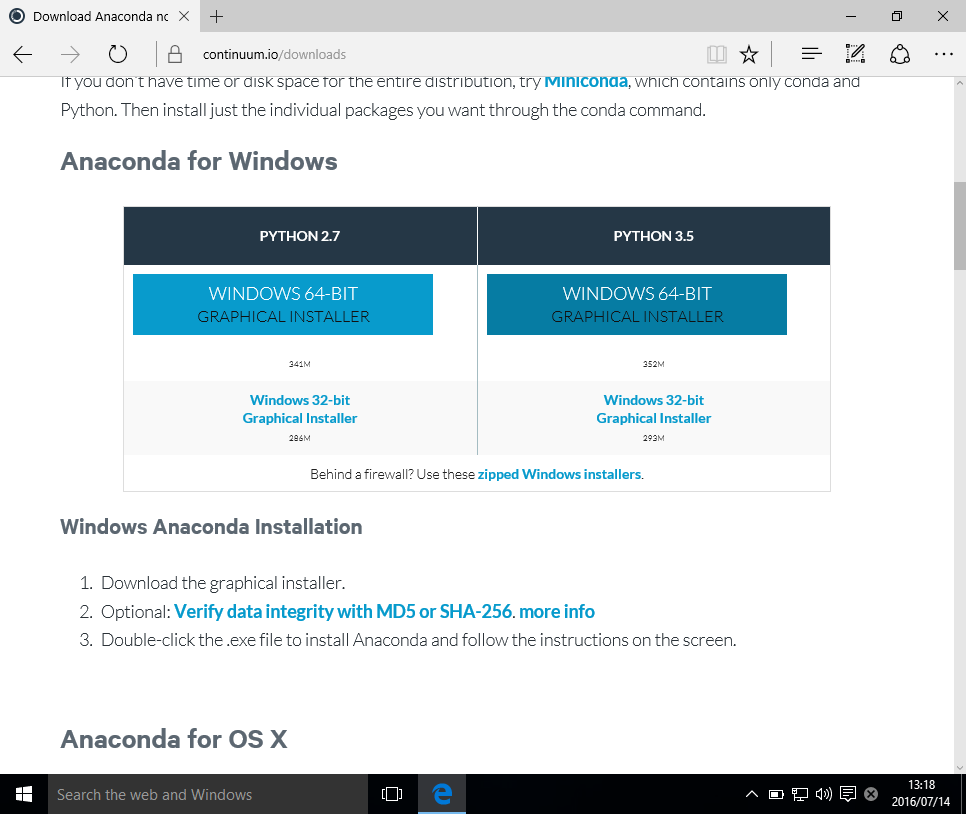
\includegraphics[width=10cm]{TeX_files/fig_python_install/Anaconda_download.png}
	\caption{
		\label{fig:Anaconda_download}
		Anacondaのダウンロードページの様子。Windows用のPython3.5のものをダウンロードすること。
	}
\end{figure}


\section{Anacondaのインストール}
先ほどダウンロードしたファイルを実行(クリック)することでインストールが始まる。

ダウンロードしたファイルの保存場所がわからなければインターネットブラウザの設定を確認する。
多くの場合、デフォルトではダウンロードフォルダ(図\ref{fig:Anaconda_install1}参照)にダウンロードされる。

インストーラにはいくつか質問されるが、よくわからなければデフォルトのままでよい。

\begin{figure}
	\centering
	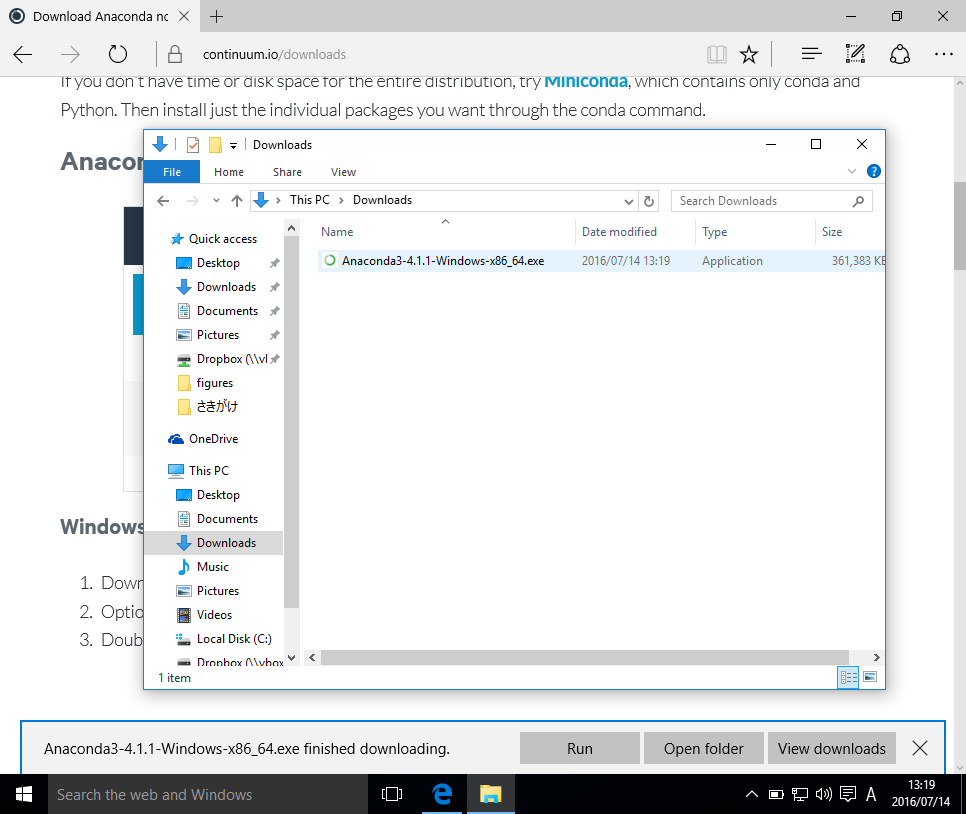
\includegraphics[width=10cm]{TeX_files/fig_python_install/Anaconda_install.png}
	\caption{
		\label{fig:Anaconda_install1}
		ダウンロードした場所をエクスプローラで開き、ファイルを実行する。
	}
\end{figure}

\begin{figure}
	\centering
	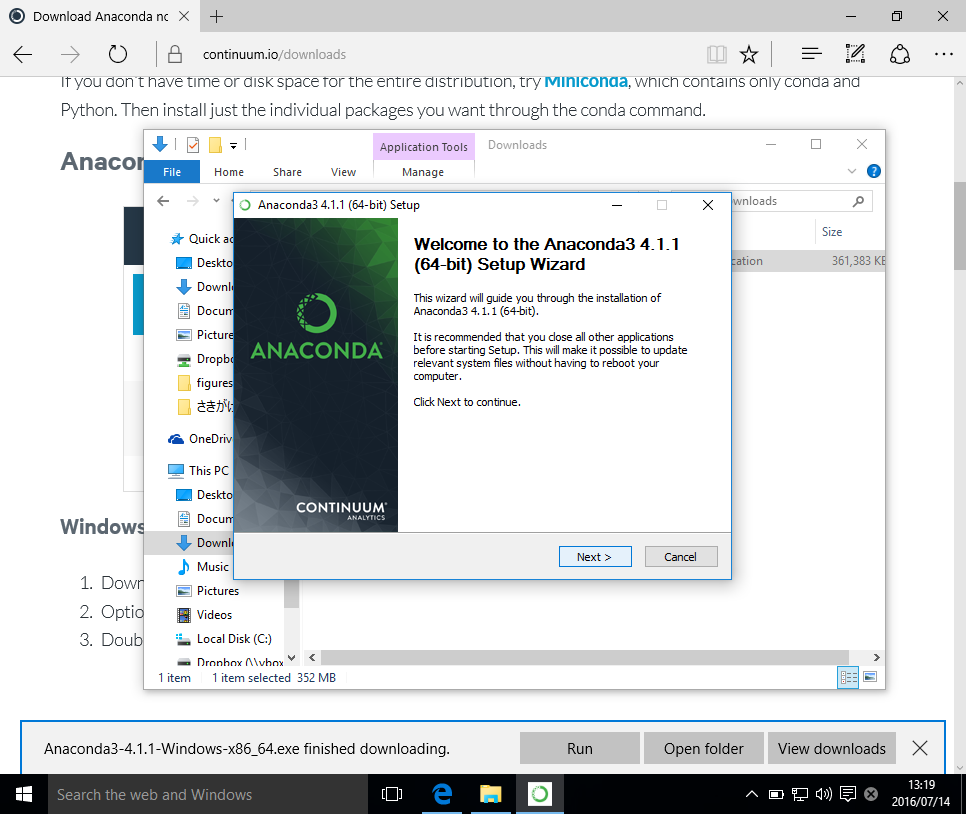
\includegraphics[width=10cm]{TeX_files/fig_python_install/Anaconda_install2.png}
	\caption{
		\label{fig:Anaconda_install2}
		インストーラを実行した時の様子。
	}
\end{figure}

\begin{figure}
	\centering
	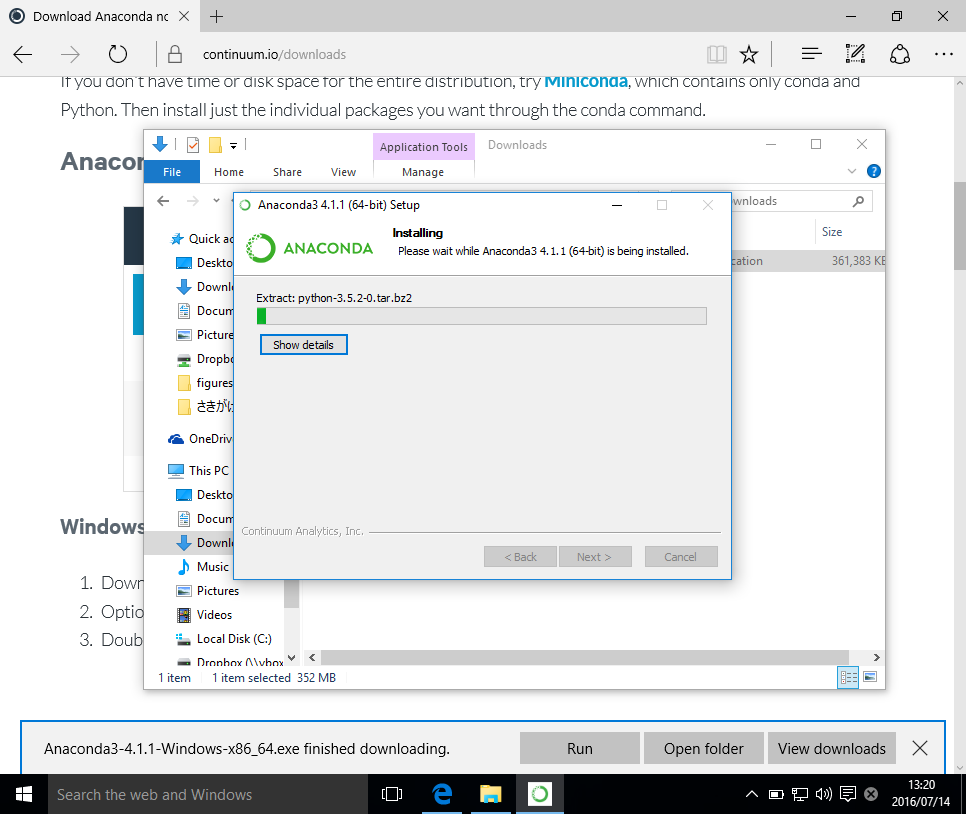
\includegraphics[width=10cm]{TeX_files/fig_python_install/Anaconda_install3.png}
	\caption{
		\label{fig:Anaconda_install3}
		インストールには少し時間がかかる。
	}
\end{figure}

\begin{figure}
	\centering
	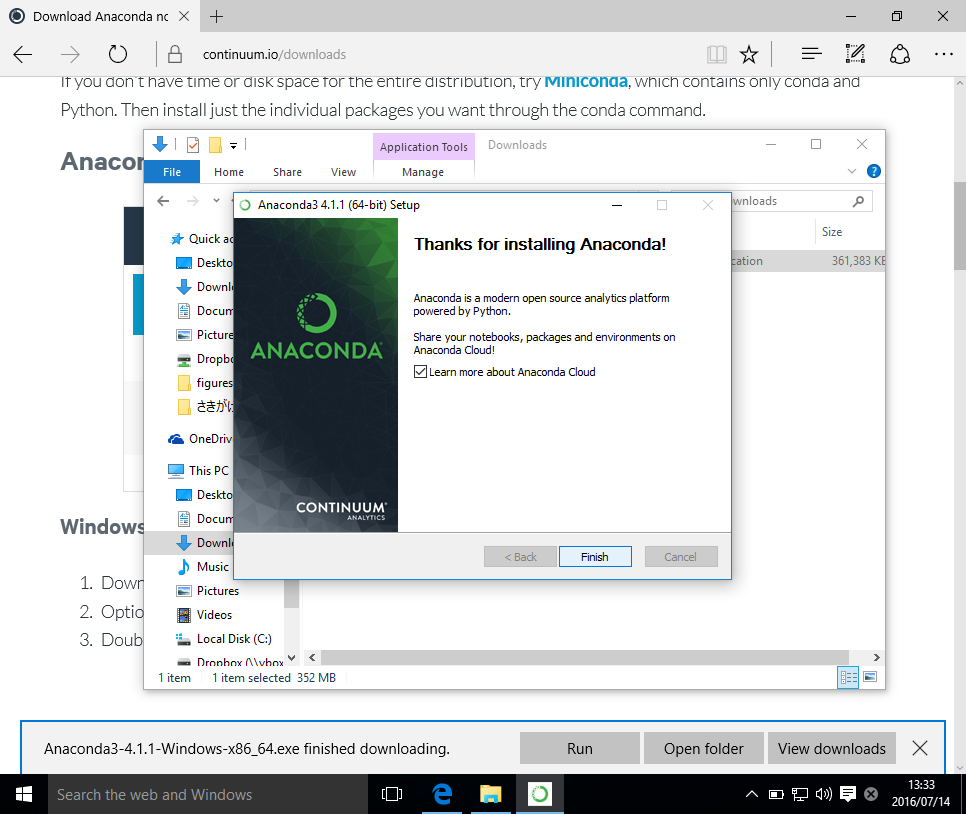
\includegraphics[width=10cm]{TeX_files/fig_python_install/Anaconda_install5.png}
	\caption{
		\label{fig:Anaconda_install5}
		このような画面が出れば完成である。
	}
\end{figure}

\chapter{対話型数値計算}

本章の目的は、
Pythonの対話型実行環境であるJupyter-notebookを用いてコンピュータによる数値計算を体感し、プログラミングの原理を実感することである。

Jupyter-notebookは、データ解析を簡単に実施できること、その結果を再利用かつ配布しやすい形で残すことができるため、現在急激に利用が広まっているソフトウェアである。

インストールも簡単であるため、各自のPCにもインストールすることを勧める。詳しくは、\ref{chap:anaconda}章を参照すること。

\section{Jupyter-notebookの起動}
Jupyte起動するためにコマンドプロンプトを実行する。
いくつか方法があるが「Winキー」+「R」を同時押しして「ファイル名から起動」を実行し、

\url{cmd}

\noindent を入力しEnterを押す方法が簡単である(図\ref{fig:Anaconda_launch1})。
コマンドプロンプトで

\url{jupyter-notebook}

\noindent を入力し実行すると(図\ref{fig:Anaconda_launch2})、
Jupyter-notebookのスタート画面が立ち上がる(図\ref{fig:Anaconda_launch3})。
 
\begin{figure}[htbp]
	\centering
	\fbox{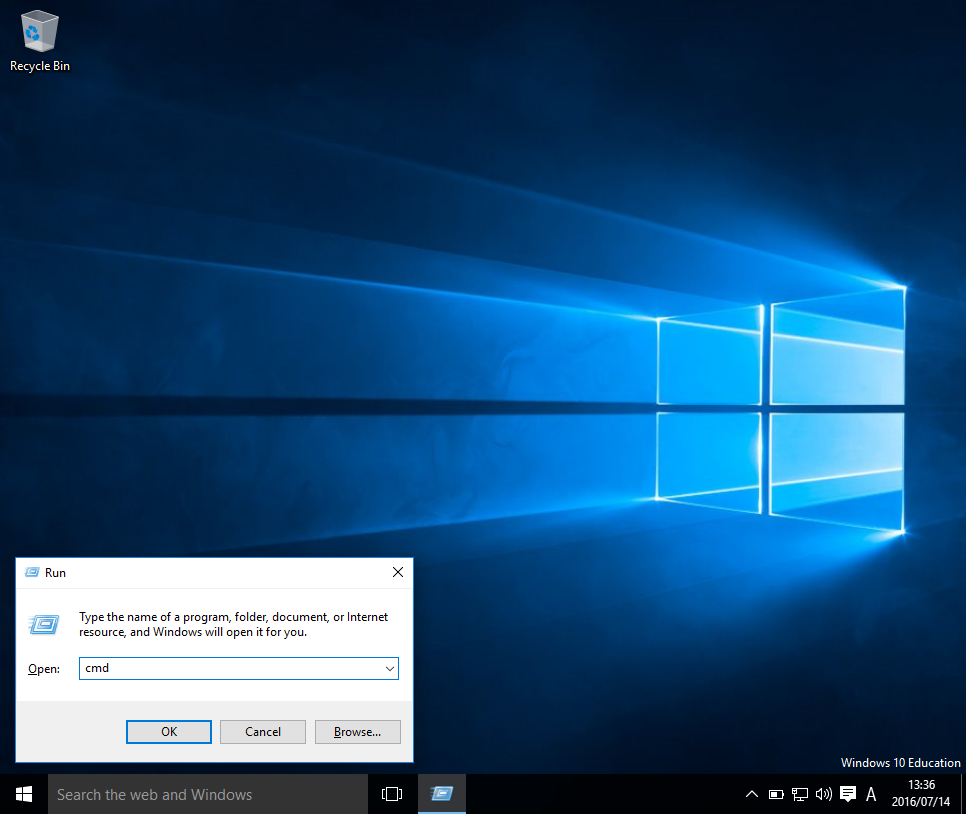
\includegraphics[width=10cm]{TeX_files/fig_python_install/Anaconda_launch1.png}}
	\caption{
		\label{fig:Anaconda_launch1}
		「Winキー」+「R」を押して出てくる検索窓に「cmd」を入力してEnterを押す。
			}
\end{figure}

\begin{figure}[htbp]
	\centering
	\fbox{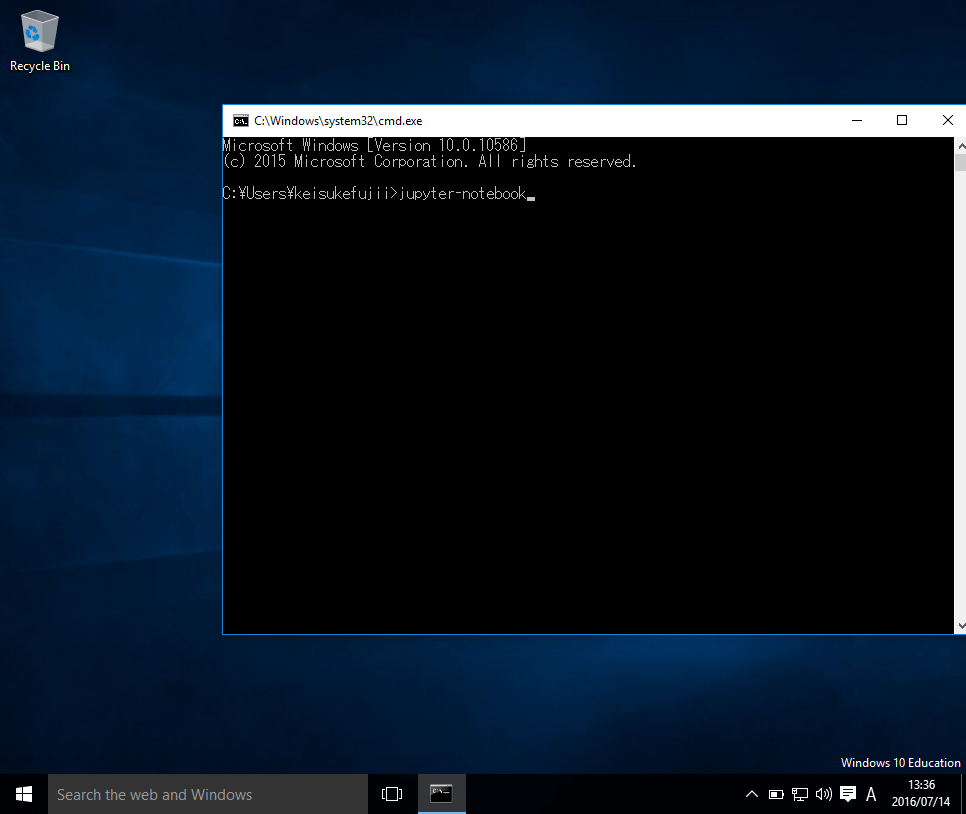
\includegraphics[width=10cm]{TeX_files/fig_python_install/Anaconda_launch2.png}}
	\caption{
		\label{fig:Anaconda_launch2}
		コマンドプロンプト内で「Jupyter-notebook」と入力し実行する。
	}
\end{figure}

\begin{figure}[htbp]
	\centering
	\fbox{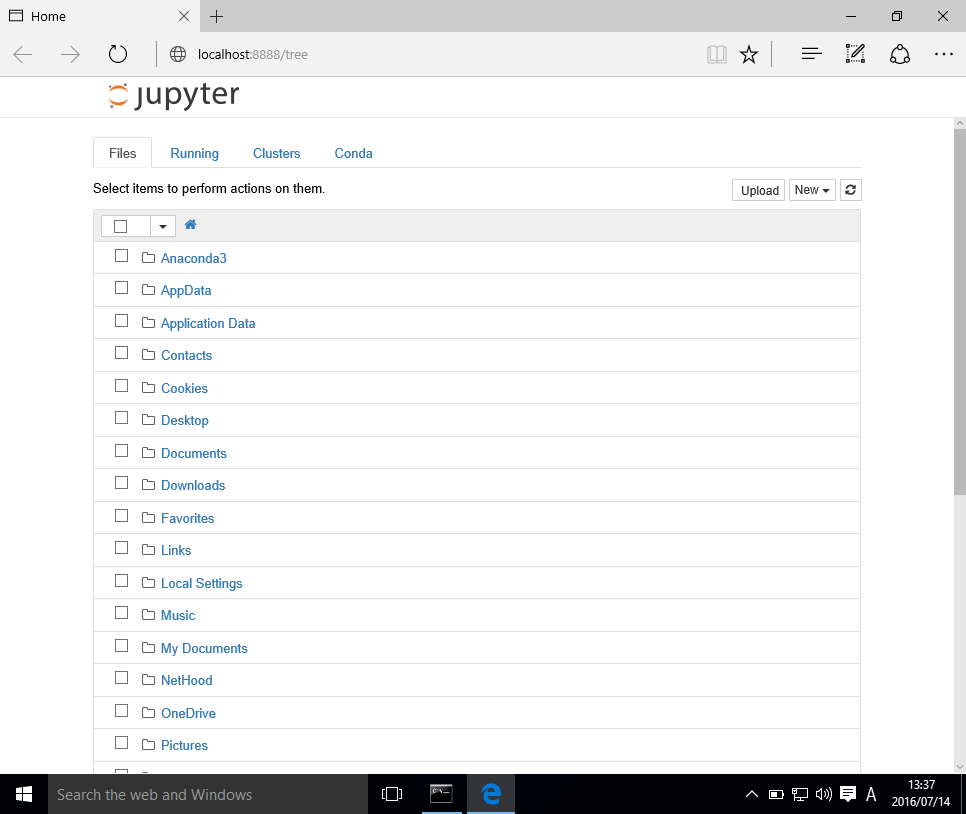
\includegraphics[width=10cm]{TeX_files/fig_python_install/Anaconda_launch3.png}}
	\caption{
		\label{fig:Anaconda_launch3}
		Jupyter-notebookの起動画面の一例。
	}
\end{figure}



% % % % % % % % % % % % % % % % % % % % % % % % % % % % % % % % % % % % % %


\section{Jupyer-notebookファイルの作成}
本演習を含め、将来的にはJupyter-notebookファイルを大量に作成することになる。
作成したファイルを見つけやすくするために、フォルダ構造を整理する。

マイドキュメント フォルダの中に、Johokiso-enshuフォルダを作成する。
マイドキュメントフォルダをクリックしその中に移動したあと、NewボタンからFolderをクリックする。
作成したフォルダの左側のチェックボックスをクリックすると出てくる renameボタンを押すことで名前の変更ができる(図\ref{fig:Jupyter_launch1})。

Johokiso-enshuフォルダ内に移動し、NewボタンからPython 3を起動する。
新しいウィンドウが開く(図\ref{fig:Jupyter_launch2})。



\begin{figure}[htbp]
	\centering
	\fbox{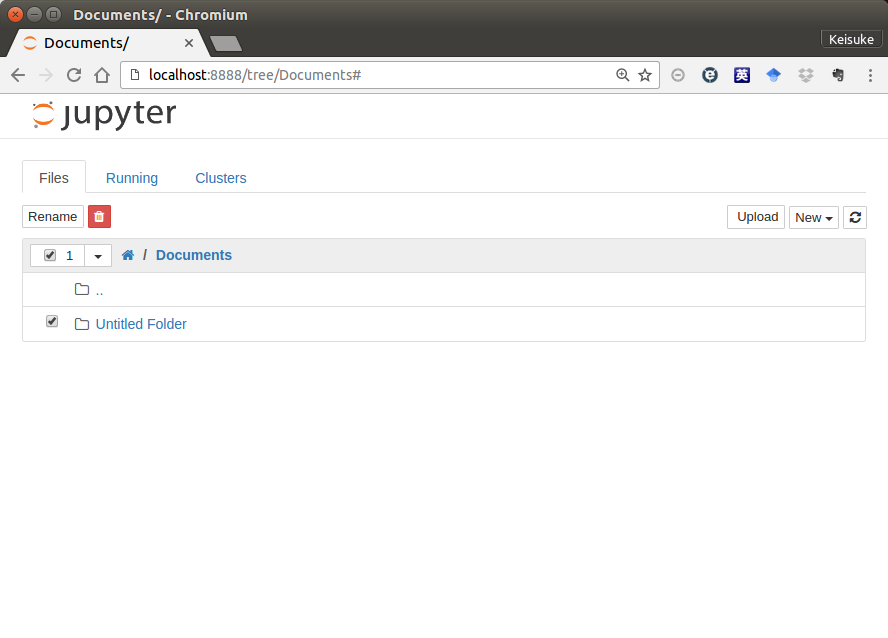
\includegraphics[width=10cm]{TeX_files/fig_python_install/Jupyter-launch1.png}}
	\caption{
		\label{fig:Jupyter_launch1}
		Jupyter-notebookでフォルダ構造を整理する。フォルダ名左横のチェックボックスを押すと、{\ttfamily rename}ボタンが出てくる。
	}
\end{figure}




% % % % % % % % % % % % % % % % % % % % % % % % % % % % % % % % % % % % % %

\section{Jupyter-notebookの基本的な使用方法}
\subsection{ノートブック名の変更}
新しいノートブックファイルには名前がまだつけられていないので、名前を変更する。
Jupyerロゴの横のUntitledをクリックすることで名を変更できる。
今日はプログラミング1回目なので Programming1-start とする(図\ref{fig:Jupyter1})。

\begin{figure}[htbp]
	\centering
	\fbox{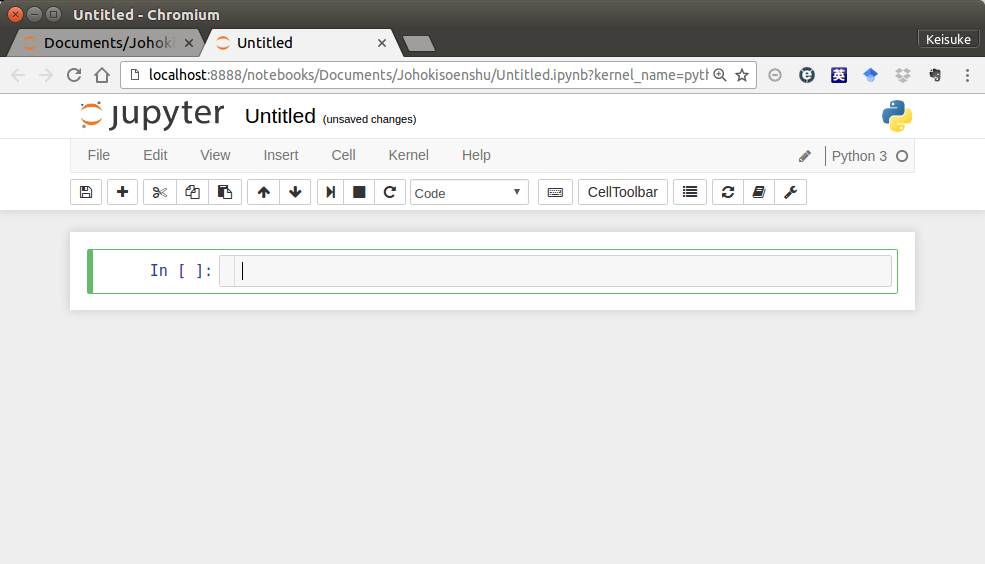
\includegraphics[width=10cm]{TeX_files/fig_python_install/Jupyter_launch2.png}}
	\caption{
		\label{fig:Jupyter_launch2}
		Jupyter-notebookで新しいPythonノートブックファイルを作成したときの様子。
	}
\end{figure}

\begin{figure}[htbp]
	\centering
	\fbox{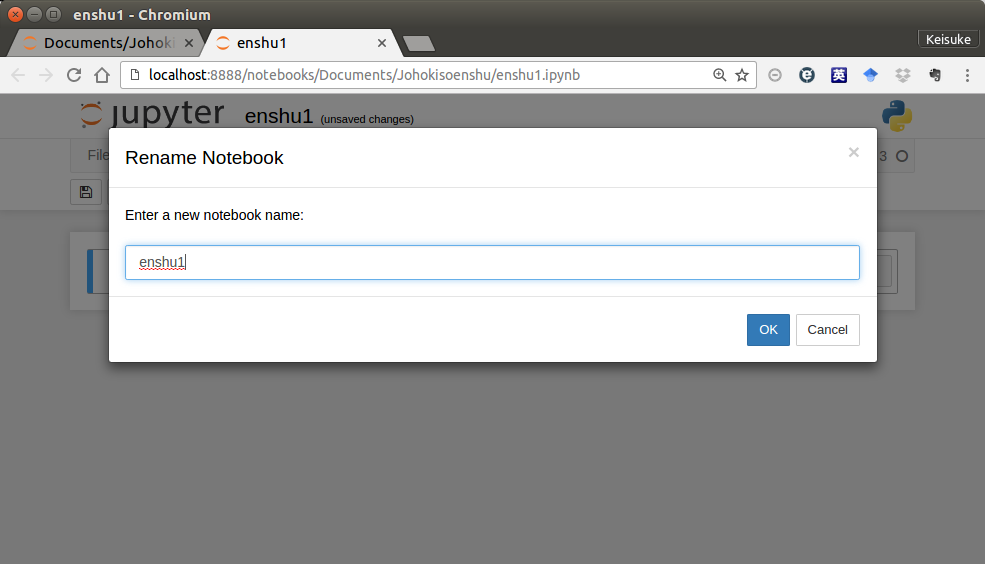
\includegraphics[width=10cm]{TeX_files/fig_python_install/Jupyter1.png}}
	\caption{
		\label{fig:Jupyter1}
		Jupyter-notebookファイルの名前を変更する。
	}
\end{figure}


% % % % % % % % % % % % % % % % % % % % % % % % % % % % % % % % % % % % % % % % % % % % % % % % % % % %

\subsection{Jupyter-notebookでの対話的プログラミング}
習うより慣れろということで、まずは命令(スクリプト)を実行させてみよう。
図\ref{fig:hello_world}にあるように、

{\ttfamily print('Hello world')}

\noindent
とセル内入力し、Shift + Enterの同時押しをするか、ツールバーの実行ボタンを押す。

エラーなく実行される場合、{\ttfamily Hello world'} とセルの下に表示されるはずである。
エラーがある場合は、図\ref{fig:hello_world_error}のように、セルの下にエラーメッセージが表示される。
このような場合は、再度正しいスクリプトを入力し、実行する。

\begin{figure}[htbp]
	\centering
	\fbox{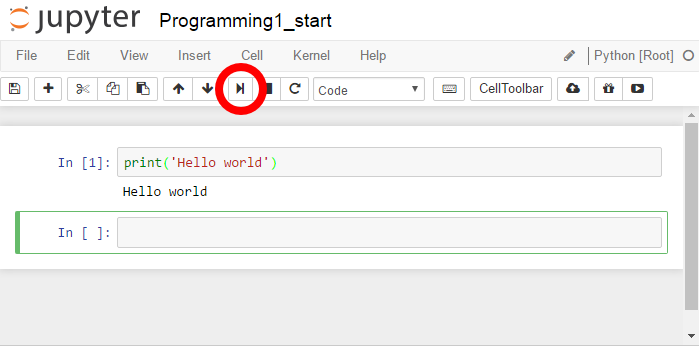
\includegraphics[width=8cm]{TeX_files/figs_jupyter_start/helloworld.png}}
	\caption{
		\label{fig:hello_world}
		{\ttfamily print('Hello world')} コマンドの実行画面
	}
\end{figure}
\begin{figure}[htbp]
	\centering
	\fbox{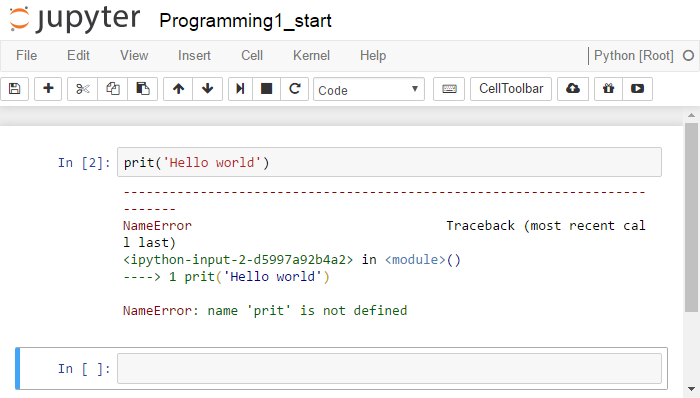
\includegraphics[width=8cm]{TeX_files/figs_jupyter_start/helloworld_error.png}}
	\caption{
		\label{fig:hello_world_error}
		コマンドを誤って入力した例。
	}
\end{figure}

この{\ttfamily print()}文は、カッコ内のものを画面に表示せよ、という命令である。
正しく入力できた時は、その結果が表示されていることがわかる。

% % % % % % % % % % % % % % % % % % % % % % % % % % % % % % % % % % % % % % % % % % % % % % % %

次に、図\ref{fig:python_start}のように一連の命令を実行してみよう。
\begin{figure}[htbp]
	\centering
	\fbox{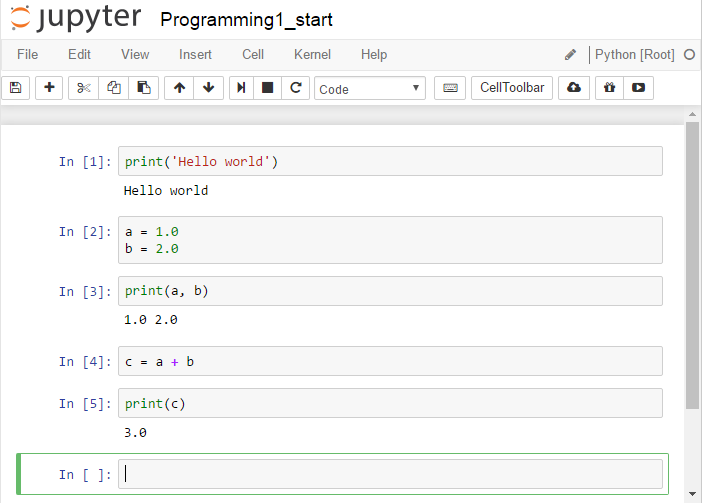
\includegraphics[width=8cm]{TeX_files/figs_jupyter_start/python_start.png}}
	\caption{
		\label{fig:python_start}
		{\ttfamily Hello world} 一連の命令を実行させた例。
	}
\end{figure}

\begin{itemize}
\item {\ttfamily a = 1.0, b = 2.0} 	

変数{\ttfamily a} に値1.0 を、変数{\ttfamily b}に値2.0 を代入する。

\item {\ttfamily print(a, b)} 	

変数{\ttfamily a, b} の値を表示する。

\item {\ttfamily c = a + b} 	

変数{\ttfamily c}に{\ttfamily a + b}を計算した結果を代入する。

\item {\ttfamily print(c)} 	

変数{\ttfamily c}の値を表示する。


\end{itemize}
\noindent
命令の内容は後で学ぶ。今は、コンピュータに命令をし、その命令が正しければコンピュータがそれを実行することがわかれば十分である。

\begin{comment}

\end{comment}
% % % % % % % % % % % % % % % % % % % % % % % % % % % % % % % % % % % % % % % % % % % % % % % % % % % %

\subsection{セルタイプ〜Code,Markdown〜}
Jupyter-notebookのセルには、{\ttfamily Code, Markdown、Raw NBConvert}の3状態がある。
これは、画面上部メニューの{\ttfamily Cell -> Cell Type}から設定できる(図\ref{fig:Cell_type})。
\begin{itemize}
\item {\ttfamily Code}状態は、上記のようなコンピュータへの命令を記入するためのもの、
\item {\ttfamily Markdown}状態は、命令以外の文章、特にコードの説明を記入するものである。
\end{itemize}

\noindent
{\ttfamily Code}状態はコンピュータへの命令内容を記述するためにもちろん重要であるが、
{\ttfamily Markdown}状態も、後でノートブックの内容を理解するために重要である。

Markdownセルを作成し、図\ref{fig:markdown}と同じ内容を記入して実行してみよ。


\begin{figure}[htbp]
	\centering
	\fbox{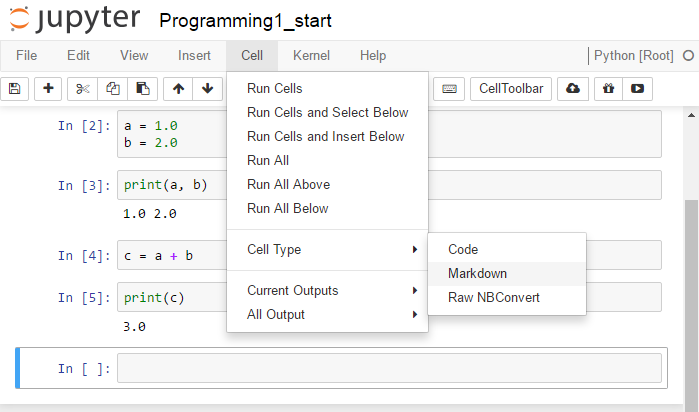
\includegraphics[width=8cm]{TeX_files/figs_jupyter_start/cell_type.png}}
	\caption{
		\label{fig:Cell_type}
		セルタイプを変更する様子。
	}
\end{figure}
\begin{figure}[htbp]
	\centering
	\fbox{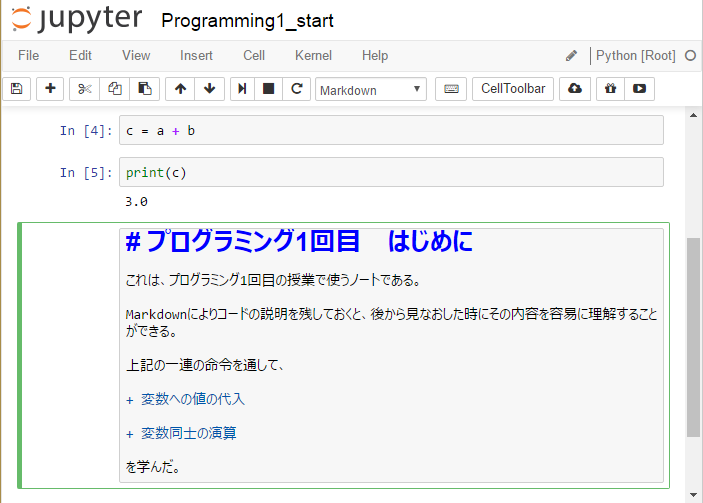
\includegraphics[width=8cm]{TeX_files/figs_jupyter_start/markdown.png}}
	\caption{
		\label{fig:markdown}
		Markdownセルに入力している様子。
	}
\end{figure}




% % % % % % % % % % % % % % % % % % % % % % % % % % % % % % % % % % % % % % % % % % % % % % % % % % % %

\subsection{Jupyter-notebookファイルの保存}
Jupyter-notebookファイルを保存するためには、左上の{\ttfamily File -> Save and Checkpoint}を選ぶか、
単純に左側のフロッピーディスクボタンをクリックする。

\subsection{Jupyter-notebookの終了}
上で作成したJupyter-notebookを保存し、ブラウザを閉じよ。
しかし実は、ブラウザを閉じただけでは実はソフトウェアは終了していない。
特に、ファイル一覧の画面で色がついたノートブックファイルは現在実行中のものを示している。

Jupyter-notebookを完全に終了させるためには、コマンドプロンプドに戻り、Ctrl+Cを押す。

% % % % % % % % % % % % % % % % % % % % % % % % % % % % % % % % % % % % % % % % % % % % % % % % % % % %
\begin{comment}
\subsection{編集モード・コマンドモード}
Jupyter-notebookには{\ttfamily 編集モード、コマンドモード}の2つのモードがある。

セル内をクリックすると文字入力が可能となる。
この時、セルの左側は緑色になるが、
これが編集モードであり、各種命令文を打ち込むことが可能である。

セル外をクリックすると、セルの左側が青色のコマンドモードになる。
この時は命令を打ち込むことはできず、その代わりキーボードからの入力が

\begin{itemize}
\item コマンドモード
セルのサイドが青くなる。文字入力はできない。
セル内をクリックするか、Enterキーを押すことで編集モードに移行できる。
このモードではショートカットでいろいろな操作が可能である。
このモードで {\ttfamily h} キーを押すことでその一覧を見ることができる。
\item 編集モード

\end{itemize}

% % % % % % % % % % % % % % % % % % % % % % % % % % % % % % % % % % % % % % % % % % % % % % % % % % % %
\section{Jupyter-notebookの活用例\label{sec:jupyter_example}}

内容の詳しい説明は後に述べることとして、実際の活用例に近いものを作成してみよう。

Jupyter-notebookを再度起動し、新しくノートブックファイルを作成する。
ファイル名は{\ttfamily Programming1-example}としておこう。
そのノートブック内で、図\ref{fig:jupyter_application}に示す一連の命令を実行せよ。

これは、物理学実験などで得られた(仮想的な)データの内容の記録、およびその可視化を行っている例である。
Jupyter-notebookでは、データがどのようにして得られたか、どのように解析したかやその結果を記録することができる。
このような情報を残しておくことで、レポート作成をスムースに行うことができる。

\begin{figure}[htbp]
	\centering
	%\fbox{\includegraphics[width=8cm]{TeX_files/figs_jupyter_start/jupyter_application.png}}
	\caption{
		\label{fig:jupyter_application}
		{\ttfamily Hello world} 一連の命令を実行させた例。
	}
\end{figure}



% % % % % % % % % % % % % % % % % % % % % % % % % % % % % % % % % % % % % % % % % % % % % % % % % % % %

\end{comment}
\chapter{Python入門}

この章では、プログラミング言語の一つであるPythonの基本的な使い方を学ぶ。
プログラミングスキルを上達させるコツは、たくさんのコードを書くことである。
以下に示すコードは全てJupyter-notebookで実行させること。





\section{\ref{sec:jupyter_example}章の内容の学習}

この章では、前章\ref{sec:jupyter_example}で入力した内容について学ぶ。
それを通して、前回とは異なるデータに対して同様の処理を行えるよう、プログラミングの基礎を学ぶ。

%TODO


\section{プログラミングの基礎}

\subsection{変数の型\label{subsec:type}}

プログラミング基礎知識の中で最も重要な概念が「変数の型」である。

「型」は変数の役割を区別するものである。

Pythonにデフォルトで用意されている型には以下のようなものがある。
\begin{itemize}
	\item {\ttfamily int} 整数を表す。
	\item {\ttfamily float} 実数を表す。
	\item {\ttfamily bool} 真・偽の2値を表す。
	\item {\ttfamily str} 文字列を表す。
	\item {\ttfamily list, dict, tuple} 複数の要素から成る変数の組を表す。
\end{itemize}

これらの役割はおいおい明らかになるとして、
まずはいろいろな変数の型を調べてみよう。

%%%%%%%%%%%%%%%%%%%%%%%%%%%%%%%%%%%%%%%%%%%%%%%%%%%%%%%

{\bfseries 課題\ref{subsec:type}}

\noindent
カッコの中の変数(引数:ひきすう と言う)の型を返す関数である{\ttfamily type()}関数を用いた以下の命令を実行せよ。
なお、ここでは、{\ttfamily print()}関数の引数に{\ttfamily type()}関数の値を代入することで、その結果を画面に表示している。


\begin{itemize}
	{\ttfamily 
		\item value\_float = 1.0

		print(type(value\_float))

		\item value\_str = 'Hello world'

		print(type(value\_str))
		
		\item value\_list = [0.1, 0.2, 3.0]
		
		print(type(value\_list))
	}
\end{itemize}

%%%%%%%%%%%%%%%%%%%%%%%%%%%%%%%%%%%%%%%%%%%%%%%%%%%%%%%

\subsubsection{int, float型\label{subsubsec:int-float}}
{\ttfamily int, float}は、数を表す型である。
int や float の例としては以下のような例がある。


{\bfseries 課題\ref{subsubsec:int-float}}

\noindent
以下の命令について、その値および型を表示させるとともに、その意味を答えよ。
必要であれば
%TODO
を参考にすること。

なお、命令の意味については、実行セルの直下にMarkdownセルを作成して記入すること。
\begin{comment}
\begin{enumerate}
	{\ttfamily 
		\item a = 2.0\\
			  b = 3.0 ** 2.0\\
		
		\item a = 5 \% 2\\
		
		\item a = 3 * 2.0 + 1.0\\
	}
\end{enumerate}
content...
\end{comment}


\subsubsection{str型\label{subsubsec:str}}
{\ttfamily str}は、文字列を表す型である。
文字列は以下のように用いることができる。

{\bfseries 課題\ref{subsubsec:str}}
以下の命令を実行せよ。



以下のような結果が
\begin{itemize}
	{\ttfamily \item float} ← 浮動小数点。実数を表す。
	{\ttfamily \item int} ← 整数
	{\ttfamily \item str} ← 文字列
\end{itemize}

なお、オブジェクト指向と呼ばれる現代的なプログラミング技法では、
型の設計が開発の中心的役割を担う。

オブジェクト指向プログラミングについては、本授業の最後に少し触れる。


と表示されたはずである。
なお、「←」の右側はそれぞれの意味を表す。

次に、以下を実行せよ。

\begin{itemize}
	{\ttfamily 
		\item d = [1.0, 2.0, 3.0]
		
		print(type(d))
		
		\item print(d[0], d[1], d[2])
				
		\item print(type(d[0]))
		
		print(type(c))
	}
\end{itemize}




\subsection{}

%\chapter{対話型数値計算}


\backmatter
% bibliography, glossary and index would go here.

\section{}

\end{document}